\subsection*{\acs{tfidf}}\label{subsec:evaluation-tfidf}

The main obstacle to overcome is the high dimensionality of the \ac{tfidf} embeddings.
Hence, the goal of the parameter selection is to find a way to reduce the dimensionality of the vocabulary to 2048 
which is the maximum dense vector dimensionality of \databaseName{}.
However, the quality of the embeddings should not decline too much.

% parameter selection
The choice of the preprocessor is investigated with regard to the goal of minimizing the vocabulary size.
Both the default and a custom preprocessor are tested on a data corpus of 2048 randomly selected documents concerning the vocabulary (size).
While the default preprocessor had a vocabulary size of 5893, the custom preprocessor had a size of 5585.
The relative differences between vocabulary sizes seem to be inversely proportional to the dataset size 
since the trend is already visible for two different data corpus sizes in \autoref{tab:tfidf-preprocessor-comparison}.
The custom preprocessor is chosen because it had a smaller vocabulary size.
The differences between both vocabularies are visualized in \autoref{fig:differences-vocabularies}.

\begin{table}[!htp]
    \caption[Comparison of the default and the custom \ac{tfidf} preprocessor]
    {Comparison of vocabulary sizes resulting from the default and the custom \ac{tfidf} preprocessor on different data corpus sizes.}
    \begin{tabular}{|p{0.55\textwidth}|p{0.2\textwidth}|p{0.2\textwidth}|}
    \hline
                                                                                                    & \cellcolor[HTML]{C0C0C0}{\color[HTML]{000000} \textbf{first trial}} & \cellcolor[HTML]{C0C0C0}{\color[HTML]{000000} \textbf{second trial}} \\ \hline
    \cellcolor[HTML]{C0C0C0}{\color[HTML]{000000} \textbf{document corpus size M}}                 & {\color[HTML]{000000} 195}                                          & {\color[HTML]{000000} 2048}                                          \\ \hline
    \cellcolor[HTML]{C0C0C0}{\color[HTML]{000000} \textbf{custom preprocessor vocabulary size A}}  & {\color[HTML]{000000} 1521}                                         & {\color[HTML]{000000} 5585}                                          \\ \hline
    \cellcolor[HTML]{C0C0C0}{\color[HTML]{000000} \textbf{default preprocessor vocabulary size B}} & {\color[HTML]{000000} 1641}                                         & {\color[HTML]{000000} 5893}                                          \\ \hline
    \cellcolor[HTML]{C0C0C0}{\color[HTML]{000000} \textbf{(B-A)/M}}                                & {\color[HTML]{000000} 120/195 = 0,6153846154}                       & {\color[HTML]{000000} 308/2048 = 0,150390625}                        \\ \hline
    \end{tabular}
    \label{tab:tfidf-preprocessor-comparison}
\end{table}

\begin{figure}[!htp]%
    \centering
    \subfloat[\centering The terms only present in the vocabulary produced by the default preprocessor.]{{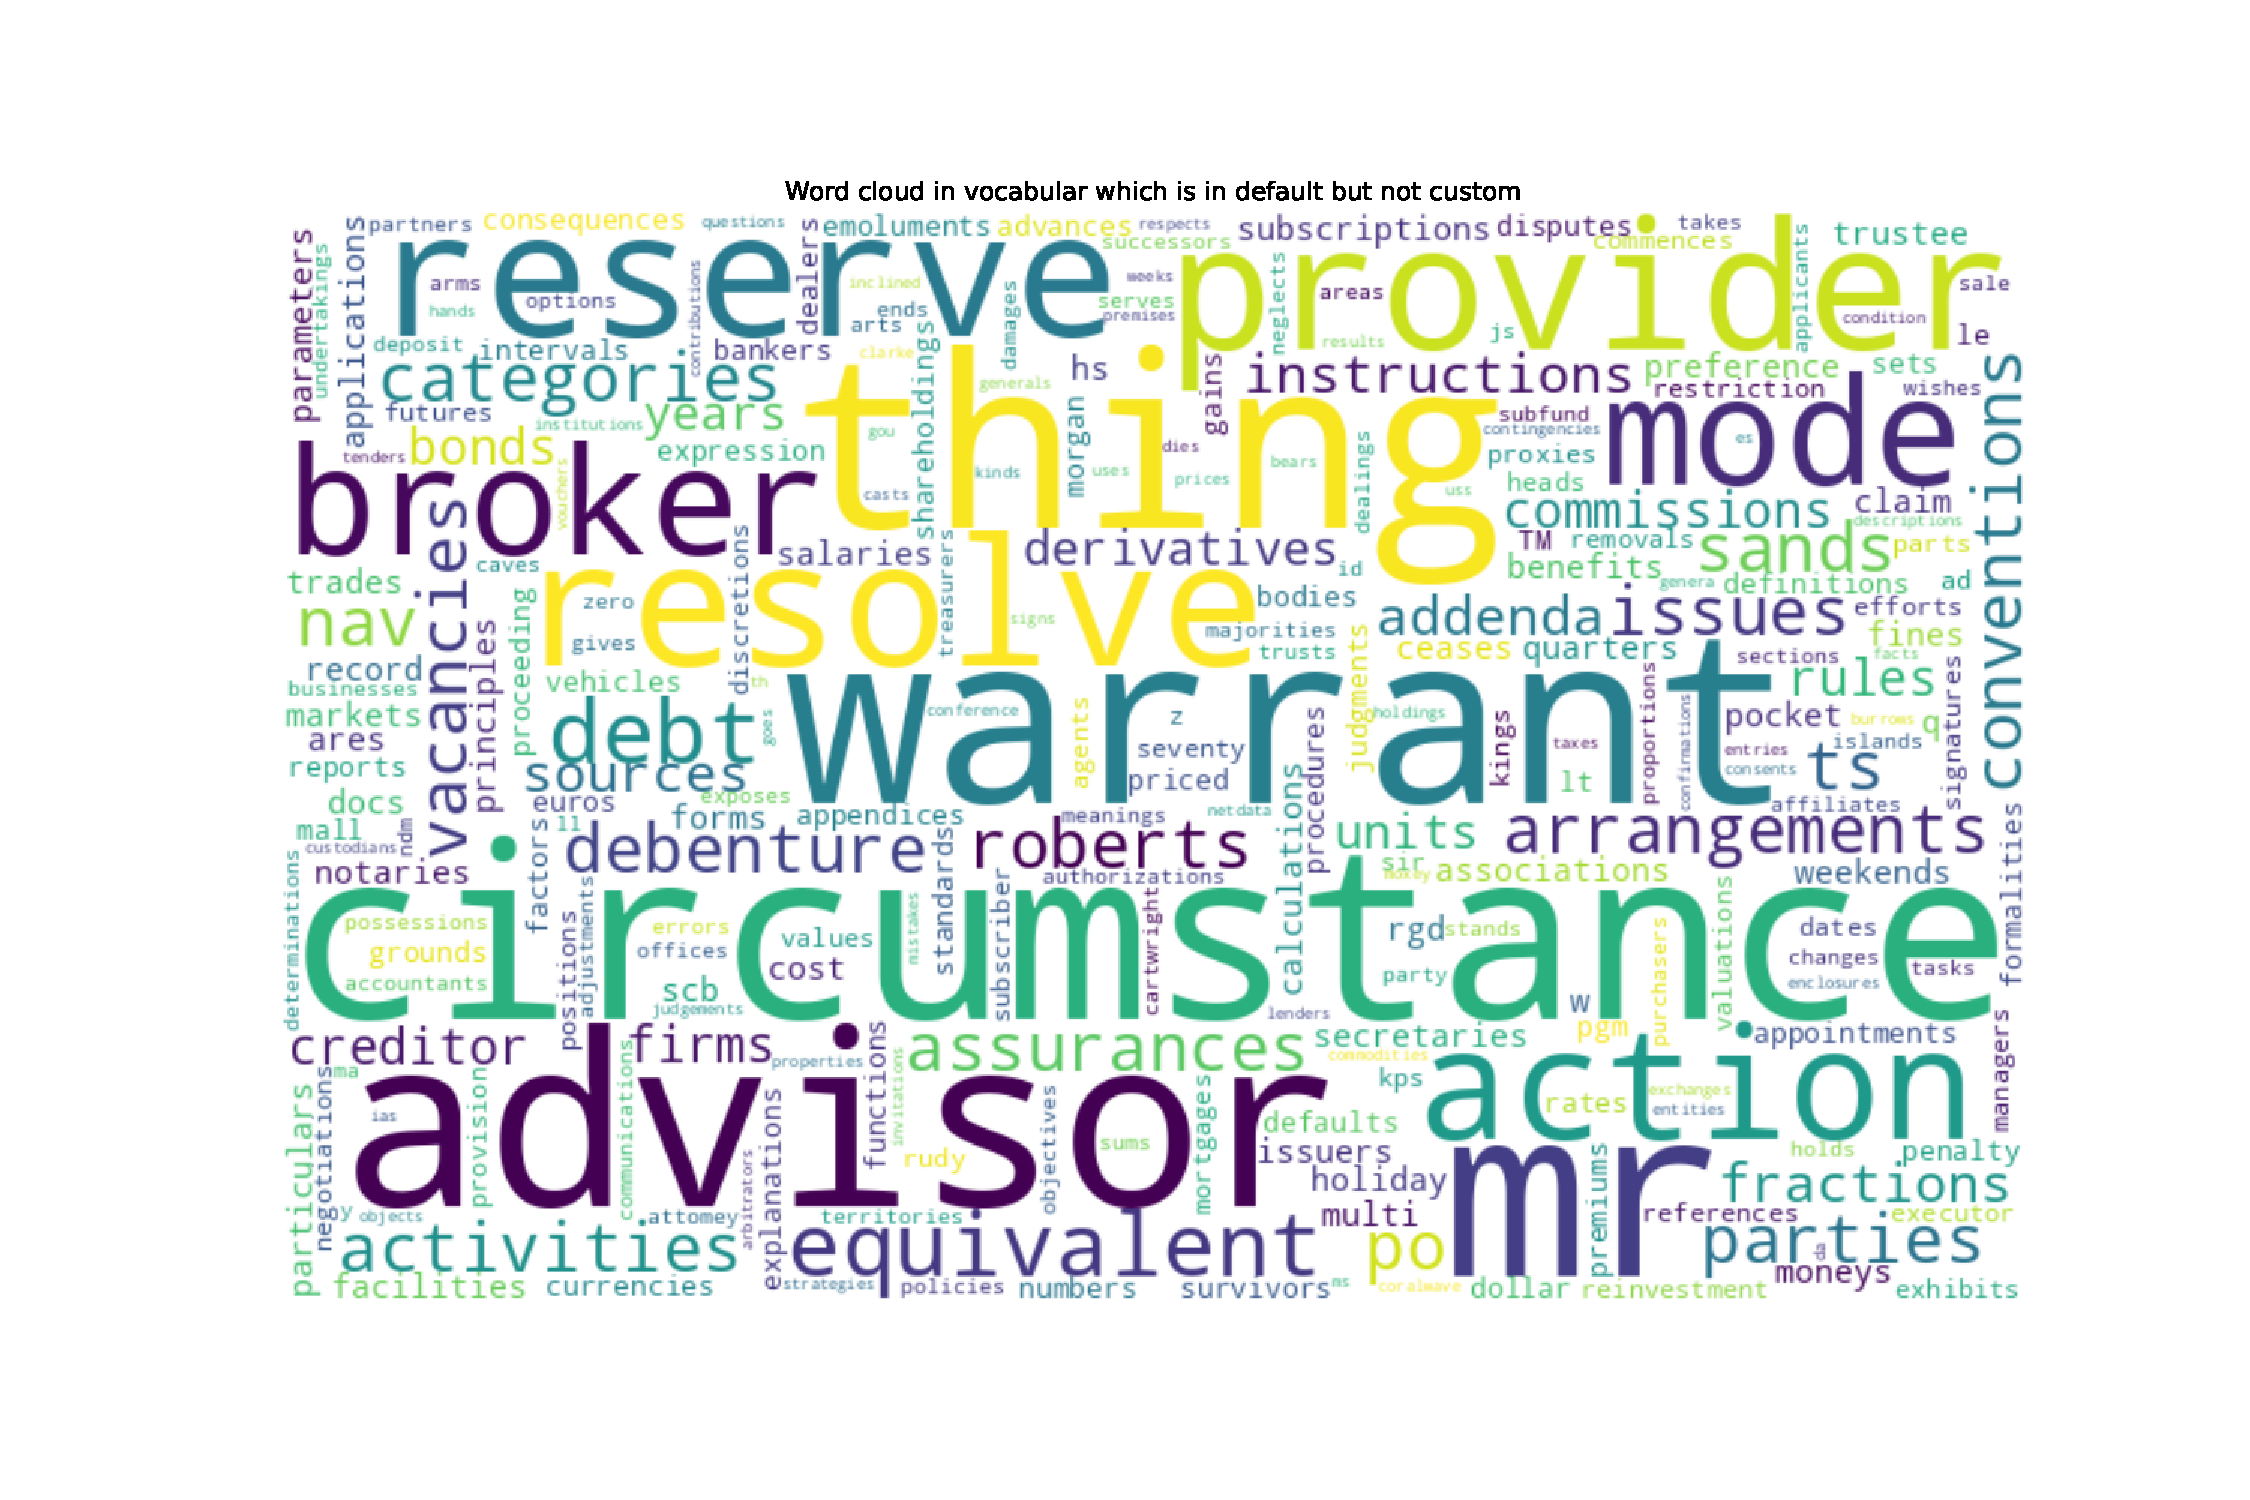
\includegraphics[width=6.8cm]{images/embeddings/tfidf/Word_cloud_in_vocabular_which_is_in_default_but_not_custom.pdf} }}%
    \qquad
    \subfloat[\centering The terms only present in the vocabulary obtained from the custom preprocessor.]{{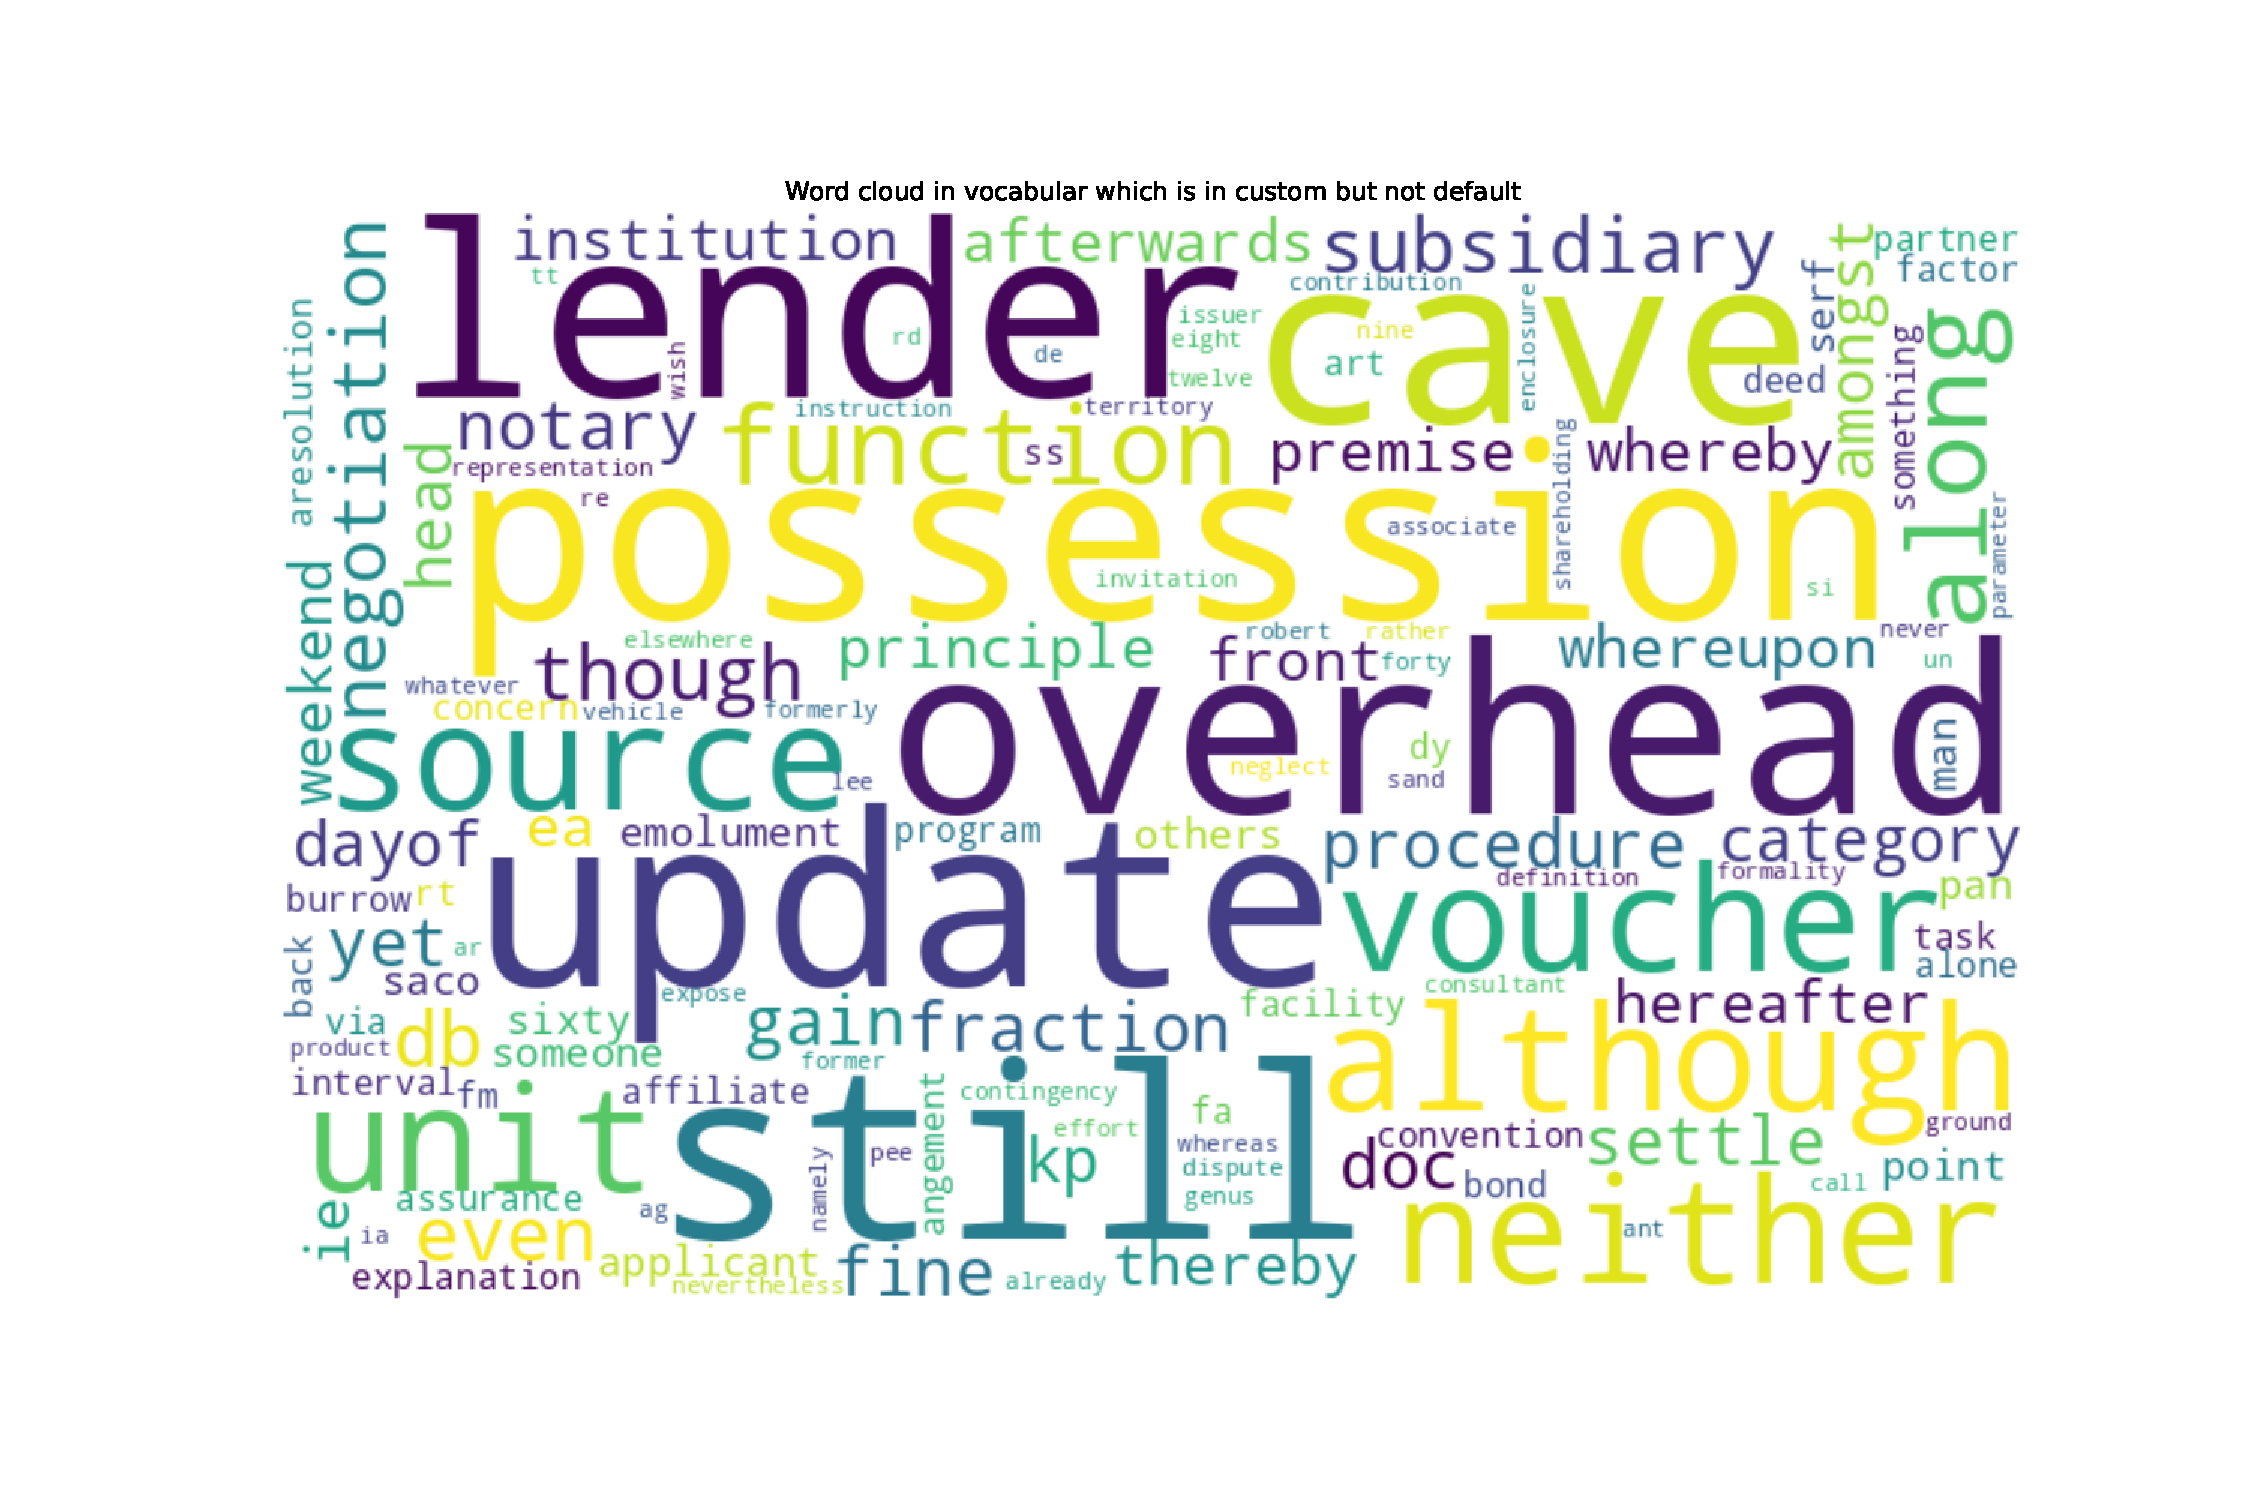
\includegraphics[width=6.8cm]{images/embeddings/tfidf/Word_cloud_in_vocabular_which_is_in_custom_but_not_default.pdf} }}%
    \caption[\wordcloud{}s for different \acs*{tfidf} preprocessors]{The \wordcloud{}s visualize which words are unique to both vocabularies 
    on a random selection of 2048 documents.}%
    \label{fig:differences-vocabularies}%
\end{figure}

As stated in \autoref{sec:eval-db}, the \ac{tfidf} embeddings can be problematic 
with regard to the dimensionality limitations imposed by \databaseName{}.
The parameters \texttt{min\_df} and \texttt{max\_df} are set to values 
which keep the vocabulary size small and thus,
the dimensionality of the embeddings is reasonably small.
Furthermore, this work employs dimensionality reduction techniques to reduce the dimensionality of the embeddings 
if the embeddings have a higher dimensionality than 2048.